\Problem
{\lr{4G EPS-AKA}}
{
در این روش پس از کامل شدن درخواست
\lr{RRC}
بین
\lr{UE}
و
\lr{eNodeB}
باعث فعال شدن
\lr{EPS-AKA}
می‌شود.
سپس یک پیام درخواست پیوست به
\lr{MME}
ارسال می‌شود.
\lr{MME}
نیز در پاسخ یک درخواست احراز اصالت شامل شناسه
\lr{IMSI}
یا همان هویت
\lr{UE}
و شناسه شبکه سرویس دهنده را به
\lr{HSS}
واقع در
\lr{Home Network}
ارسال می‌کند.

المان
\lr{HSS}
عمل رمزنگاری را بر مبنای کلید مخفی مشترک
\lr{Ki}
که میان خودش و
\lr{UE}
مشترک است انجام می‌دهد.
در نتیجه این کار یک یا چند بردار اهراز اصالت استخراج می‌شود.
در یک پیام پاسخ احراز اصالت به
\lr{MME}
ارسال می‌شود.
بردار احراز اصالت یا به اختصار
\lr{AV}
شامل یک توکن احراز اصالت به نام
\lr{AUTH}
و یک توکن پاسخ احراز اصالت هویت مورد نظر به نام
\lr{XAUTH}
است.
داده‌های دیگری نیز در این بردار وجود دارد.

\begin{figure}[H]
    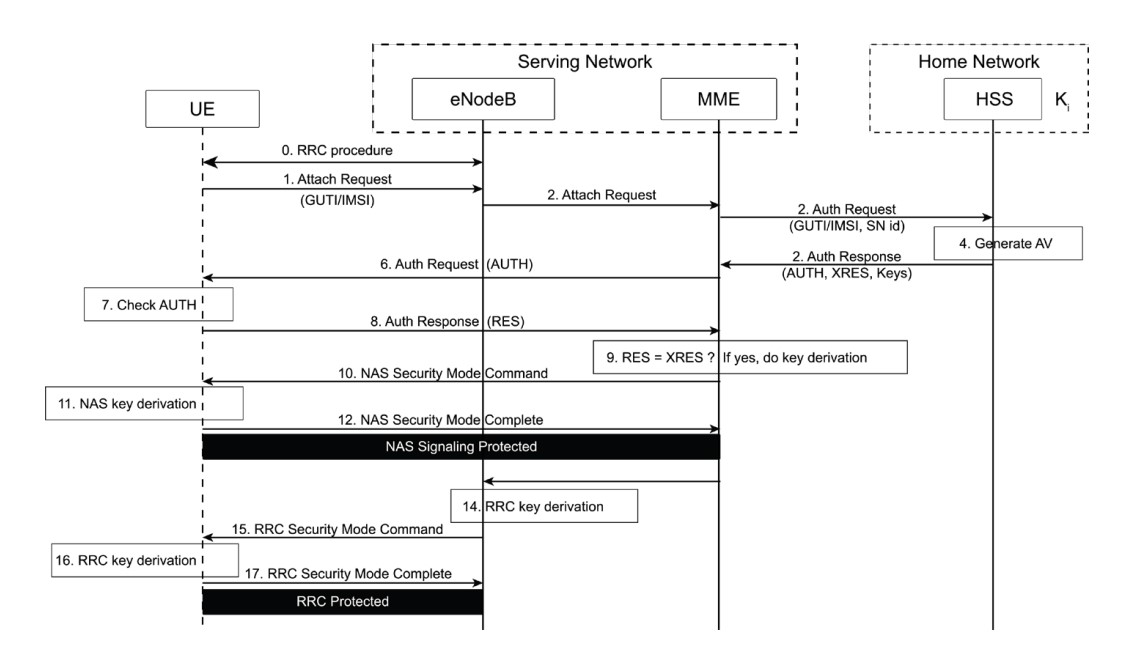
\includegraphics[width=15cm]{Images/IMG_03.jpg}
    \centering
    \caption{رویه احراز اصالت در نسل چهارم}
\end{figure}

پس از دریافت پاسخ احراز اصالت از
\lr{MME}
یک درخواست احراز اصالت از سوی
\lr{HSS}
شامل توکن
\lr{AUTH}
به
\lr{UE}
ارسال می‌شود.

\lr{UE}
این توکن را با با توکن تولید شده خودش با کلید
\lr{Ki}
مقایسه می‌کند و پس از تایید آن شبکه را قانونی حساب می‌کند و یک پاسخ احراز اصالت به
\lr{MME}
می‌فرستد.
در این پاسخ یک توکن به نام
\lr{RES}
وجود دارد که بر اساس
\lr{Ki}
تولید شده است.
\lr{MME}
این توکن را با توکن مورد انتظار خود یعنی
\lr{XRES}
مقایسه می‌کند.
در صورت برابری 
\lr{MME}
به کلید دست می‌یابد و یک دستور
\lr{Security Mode}
به
\lr{UE}
ارسال می‌کند.
سپس کلیدهایی که برای محافظت از پیام‌های سیگنالینگ
\lr{NAS}
هستند را استخراج می‌کند.
همچنین
\lr{MME}
یک کلید برای
\lr{eNodeB}
می‌فرستد که از آن کلیدهای محافظت از کانال
\lr{RRC}
به دست آمده است.
پس از اینکه
\lr{UE}
نیز کلیدهای مربوطه را به دست آورد، ارتباط بین
\lr{UE}
و
\lr{eNodeB}
امن می‌شود.
}